
%% bare_conf.tex
%% V1.4b
%% 2015/08/26
%% by Michael Shell
%% See:
%% http://www.michaelshell.org/
%% for current contact information.
%%
%% This is a skeleton file demonstrating the use of IEEEtran.cls
%% (requires IEEEtran.cls version 1.8b or later) with an IEEE
%% conference paper.
%%
%% Support sites:
%% http://www.michaelshell.org/tex/ieeetran/
%% http://www.ctan.org/pkg/ieeetran
%% and
%% http://www.ieee.org/

%%*************************************************************************
%% Legal Notice:
%% This code is offered as-is without any warranty either expressed or
%% implied; without even the implied warranty of MERCHANTABILITY or
%% FITNESS FOR A PARTICULAR PURPOSE! 
%% User assumes all risk.
%% In no event shall the IEEE or any contributor to this code be liable for
%% any damages or losses, including, but not limited to, incidental,
%% consequential, or any other damages, resulting from the use or misuse
%% of any information contained here.
%%
%% All comments are the opinions of their respective authors and are not
%% necessarily endorsed by the IEEE.
%%
%% This work is distributed under the LaTeX Project Public License (LPPL)
%% ( http://www.latex-project.org/ ) version 1.3, and may be freely used,
%% distributed and modified. A copy of the LPPL, version 1.3, is included
%% in the base LaTeX documentation of all distributions of LaTeX released
%% 2003/12/01 or later.
%% Retain all contribution notices and credits.
%% ** Modified files should be clearly indicated as such, including  **
%% ** renaming them and changing author support contact information. **
%%*************************************************************************


% *** Authors should verify (and, if needed, correct) their LaTeX system  ***
% *** with the testflow diagnostic prior to trusting their LaTeX platform ***
% *** with production work. The IEEE's font choices and paper sizes can   ***
% *** trigger bugs that do not appear when using other class files.       ***                          ***
% The testflow support page is at:
% http://www.michaelshell.org/tex/testflow/



\documentclass[conference]{IEEEtran}
% Some Computer Society conferences also require the compsoc mode option,
% but others use the standard conference format.
%
% If IEEEtran.cls has not been installed into the LaTeX system files,
% manually specify the path to it like:
% \documentclass[conference]{../sty/IEEEtran}





% Some very useful LaTeX packages include:
% (uncomment the ones you want to load)


% *** MISC UTILITY PACKAGES ***
%
%\usepackage{ifpdf}
% Heiko Oberdiek's ifpdf.sty is very useful if you need conditional
% compilation based on whether the output is pdf or dvi.
% usage:
% \ifpdf
%   % pdf code
% \else
%   % dvi code
% \fi
% The latest version of ifpdf.sty can be obtained from:
% http://www.ctan.org/pkg/ifpdf
% Also, note that IEEEtran.cls V1.7 and later provides a builtin
% \ifCLASSINFOpdf conditional that works the same way.
% When switching from latex to pdflatex and vice-versa, the compiler may
% have to be run twice to clear warning/error messages.






% *** CITATION PACKAGES ***
%
%\usepackage{cite}
% cite.sty was written by Donald Arseneau
% V1.6 and later of IEEEtran pre-defines the format of the cite.sty package
% \cite{} output to follow that of the IEEE. Loading the cite package will
% result in citation numbers being automatically sorted and properly
% "compressed/ranged". e.g., [1], [9], [2], [7], [5], [6] without using
% cite.sty will become [1], [2], [5]--[7], [9] using cite.sty. cite.sty's
% \cite will automatically add leading space, if needed. Use cite.sty's
% noadjust option (cite.sty V3.8 and later) if you want to turn this off
% such as if a citation ever needs to be enclosed in parenthesis.
% cite.sty is already installed on most LaTeX systems. Be sure and use
% version 5.0 (2009-03-20) and later if using hyperref.sty.
% The latest version can be obtained at:
% http://www.ctan.org/pkg/cite
% The documentation is contained in the cite.sty file itself.






% *** GRAPHICS RELATED PACKAGES ***
%
\ifCLASSINFOpdf
  \usepackage[pdftex]{graphicx}
  % declare the path(s) where your graphic files are
  \graphicspath{{./figures/}}
  % and their extensions so you won't have to specify these with
  % every instance of \includegraphics
  \DeclareGraphicsExtensions{.pdf,.jpeg,.png}
\else
  % or other class option (dvipsone, dvipdf, if not using dvips). graphicx
  % will default to the driver specified in the system graphics.cfg if no
  % driver is specified.
  % \usepackage[dvips]{graphicx}
  % declare the path(s) where your graphic files are
  % \graphicspath{{../eps/}}
  % and their extensions so you won't have to specify these with
  % every instance of \includegraphics
  % \DeclareGraphicsExtensions{.eps}
\fi
% graphicx was written by David Carlisle and Sebastian Rahtz. It is
% required if you want graphics, photos, etc. graphicx.sty is already
% installed on most LaTeX systems. The latest version and documentation
% can be obtained at: 
% http://www.ctan.org/pkg/graphicx
% Another good source of documentation is "Using Imported Graphics in
% LaTeX2e" by Keith Reckdahl which can be found at:
% http://www.ctan.org/pkg/epslatex
%
% latex, and pdflatex in dvi mode, support graphics in encapsulated
% postscript (.eps) format. pdflatex in pdf mode supports graphics
% in .pdf, .jpeg, .png and .mps (metapost) formats. Users should ensure
% that all non-photo figures use a vector format (.eps, .pdf, .mps) and
% not a bitmapped formats (.jpeg, .png). The IEEE frowns on bitmapped formats
% which can result in "jaggedy"/blurry rendering of lines and letters as
% well as large increases in file sizes.
%
% You can find documentation about the pdfTeX application at:
% http://www.tug.org/applications/pdftex





% *** MATH PACKAGES ***
%
\usepackage{amsmath}
% A popular package from the American Mathematical Society that provides
% many useful and powerful commands for dealing with mathematics.
%
% Note that the amsmath package sets \interdisplaylinepenalty to 10000
% thus preventing page breaks from occurring within multiline equations. Use:
%\interdisplaylinepenalty=2500
% after loading amsmath to restore such page breaks as IEEEtran.cls normally
% does. amsmath.sty is already installed on most LaTeX systems. The latest
% version and documentation can be obtained at:
% http://www.ctan.org/pkg/amsmath





% *** SPECIALIZED LIST PACKAGES ***
%
%\usepackage{algorithmic}
% algorithmic.sty was written by Peter Williams and Rogerio Brito.
% This package provides an algorithmic environment fo describing algorithms.
% You can use the algorithmic environment in-text or within a figure
% environment to provide for a floating algorithm. Do NOT use the algorithm
% floating environment provided by algorithm.sty (by the same authors) or
% algorithm2e.sty (by Christophe Fiorio) as the IEEE does not use dedicated
% algorithm float types and packages that provide these will not provide
% correct IEEE style captions. The latest version and documentation of
% algorithmic.sty can be obtained at:
% http://www.ctan.org/pkg/algorithms
% Also of interest may be the (relatively newer and more customizable)
% algorithmicx.sty package by Szasz Janos:
% http://www.ctan.org/pkg/algorithmicx




% *** ALIGNMENT PACKAGES ***
%
%\usepackage{array}
% Frank Mittelbach's and David Carlisle's array.sty patches and improves
% the standard LaTeX2e array and tabular environments to provide better
% appearance and additional user controls. As the default LaTeX2e table
% generation code is lacking to the point of almost being broken with
% respect to the quality of the end results, all users are strongly
% advised to use an enhanced (at the very least that provided by array.sty)
% set of table tools. array.sty is already installed on most systems. The
% latest version and documentation can be obtained at:
% http://www.ctan.org/pkg/array


% IEEEtran contains the IEEEeqnarray family of commands that can be used to
% generate multiline equations as well as matrices, tables, etc., of high
% quality.




% *** SUBFIGURE PACKAGES ***
%\ifCLASSOPTIONcompsoc
%  \usepackage[caption=false,font=normalsize,labelfont=sf,textfont=sf]{subfig}
%\else
%  \usepackage[caption=false,font=footnotesize]{subfig}
%\fi
% subfig.sty, written by Steven Douglas Cochran, is the modern replacement
% for subfigure.sty, the latter of which is no longer maintained and is
% incompatible with some LaTeX packages including fixltx2e. However,
% subfig.sty requires and automatically loads Axel Sommerfeldt's caption.sty
% which will override IEEEtran.cls' handling of captions and this will result
% in non-IEEE style figure/table captions. To prevent this problem, be sure
% and invoke subfig.sty's "caption=false" package option (available since
% subfig.sty version 1.3, 2005/06/28) as this is will preserve IEEEtran.cls
% handling of captions.
% Note that the Computer Society format requires a larger sans serif font
% than the serif footnote size font used in traditional IEEE formatting
% and thus the need to invoke different subfig.sty package options depending
% on whether compsoc mode has been enabled.
%
% The latest version and documentation of subfig.sty can be obtained at:
% http://www.ctan.org/pkg/subfig




% *** FLOAT PACKAGES ***
%
%\usepackage{fixltx2e}
% fixltx2e, the successor to the earlier fix2col.sty, was written by
% Frank Mittelbach and David Carlisle. This package corrects a few problems
% in the LaTeX2e kernel, the most notable of which is that in current
% LaTeX2e releases, the ordering of single and double column floats is not
% guaranteed to be preserved. Thus, an unpatched LaTeX2e can allow a
% single column figure to be placed prior to an earlier double column
% figure.
% Be aware that LaTeX2e kernels dated 2015 and later have fixltx2e.sty's
% corrections already built into the system in which case a warning will
% be issued if an attempt is made to load fixltx2e.sty as it is no longer
% needed.
% The latest version and documentation can be found at:
% http://www.ctan.org/pkg/fixltx2e


%\usepackage{stfloats}
% stfloats.sty was written by Sigitas Tolusis. This package gives LaTeX2e
% the ability to do double column floats at the bottom of the page as well
% as the top. (e.g., "\begin{figure*}[!b]" is not normally possible in
% LaTeX2e). It also provides a command:
%\fnbelowfloat
% to enable the placement of footnotes below bottom floats (the standard
% LaTeX2e kernel puts them above bottom floats). This is an invasive package
% which rewrites many portions of the LaTeX2e float routines. It may not work
% with other packages that modify the LaTeX2e float routines. The latest
% version and documentation can be obtained at:
% http://www.ctan.org/pkg/stfloats
% Do not use the stfloats baselinefloat ability as the IEEE does not allow
% \baselineskip to stretch. Authors submitting work to the IEEE should note
% that the IEEE rarely uses double column equations and that authors should try
% to avoid such use. Do not be tempted to use the cuted.sty or midfloat.sty
% packages (also by Sigitas Tolusis) as the IEEE does not format its papers in
% such ways.
% Do not attempt to use stfloats with fixltx2e as they are incompatible.
% Instead, use Morten Hogholm'a dblfloatfix which combines the features
% of both fixltx2e and stfloats:
%
% \usepackage{dblfloatfix}
% The latest version can be found at:
% http://www.ctan.org/pkg/dblfloatfix




% *** PDF, URL AND HYPERLINK PACKAGES ***
%
\usepackage{url}
% url.sty was written by Donald Arseneau. It provides better support for
% handling and breaking URLs. url.sty is already installed on most LaTeX
% systems. The latest version and documentation can be obtained at:
% http://www.ctan.org/pkg/url
% Basically, \url{my_url_here}.

\usepackage{adjustbox}


% *** Do not adjust lengths that control margins, column widths, etc. ***
% *** Do not use packages that alter fonts (such as pslatex).         ***
% There should be no need to do such things with IEEEtran.cls V1.6 and later.
% (Unless specifically asked to do so by the journal or conference you plan
% to submit to, of course. )


% correct bad hyphenation here
\hyphenation{op-tical net-works semi-conduc-tor}


\begin{document}
%
% paper title
% Titles are generally capitalized except for words such as a, an, and, as,
% at, but, by, for, in, nor, of, on, or, the, to and up, which are usually
% not capitalized unless they are the first or last word of the title.
% Linebreaks \\ can be used within to get better formatting as desired.
% Do not put math or special symbols in the title.
\title{Monolingual Written Natural Language Identification with Naïve Bayes and LSTMs}


% author names and affiliations
% use a multiple column layout for up to three different
% affiliations
\author{\IEEEauthorblockN{Jacob Lundberg}
\IEEEauthorblockA{Linköping University\\
LiU-id: jaclu010\\
Email: jaclu010@student.liu.se}}
%\and
%\IEEEauthorblockN{Homer Simpson}
%\IEEEauthorblockA{Twentieth Century Fox\\
%Springfield, USA\\
%Email: homer@thesimpsons.com}
%\and
%\IEEEauthorblockN{James Kirk\\ and Montgomery Scott}
%\IEEEauthorblockA{Starfleet Academy\\
%San Francisco, California 96678--2391\\
%Telephone: (800) 555--1212\\
%Fax: (888) 555--1212}}

% conference papers do not typically use \thanks and this command
% is locked out in conference mode. If really needed, such as for
% the acknowledgment of grants, issue a \IEEEoverridecommandlockouts
% after \documentclass

% for over three affiliations, or if they all won't fit within the width
% of the page, use this alternative format:
% 
%\author{\IEEEauthorblockN{Michael Shell\IEEEauthorrefmark{1},
%Homer Simpson\IEEEauthorrefmark{2},
%James Kirk\IEEEauthorrefmark{3}, 
%Montgomery Scott\IEEEauthorrefmark{3} and
%Eldon Tyrell\IEEEauthorrefmark{4}}
%\IEEEauthorblockA{\IEEEauthorrefmark{1}School of Electrical and Computer Engineering\\
%Georgia Institute of Technology,
%Atlanta, Georgia 30332--0250\\ Email: see http://www.michaelshell.org/contact.html}
%\IEEEauthorblockA{\IEEEauthorrefmark{2}Twentieth Century Fox, Springfield, USA\\
%Email: homer@thesimpsons.com}
%\IEEEauthorblockA{\IEEEauthorrefmark{3}Starfleet Academy, San Francisco, California 96678-2391\\
%Telephone: (800) 555--1212, Fax: (888) 555--1212}
%\IEEEauthorblockA{\IEEEauthorrefmark{4}Tyrell Inc., 123 Replicant Street, Los Angeles, California 90210--4321}}




% use for special paper notices
%\IEEEspecialpapernotice{(Invited Paper)}




% make the title area
\maketitle

% As a general rule, do not put math, special symbols or citations
% in the abstract
\begin{abstract}
This project aims to correctly classify the language of written text paragraphs. Given a paragraph, one out of 235 languages can be classified. Chosen model solutions to the classification problem is an Naïve Bayes model and an LSTM. They reach a classification accuracy of 94\% and 78\% respectively. This is a lot better that the authors proposed method, achieving an accuracy of 88\%.
\end{abstract}

% no keywords




% For peer review papers, you can put extra information on the cover
% page as needed:
\ifCLASSOPTIONpeerreview
\begin{center} \bfseries EDICS Category: 3-BBND \end{center}
\fi
%
% For peerreview papers, this IEEEtran command inserts a page break and
% creates the second title. It will be ignored for other modes.
\IEEEpeerreviewmaketitle



\section{Introduction}
% no \IEEEPARstart
The art of identifying the language in a text jas been around a long time. It is something we humans do on a daily basis. The agent in question needs to understand what language is being read in order to interpret it correctly. It is an important part of the pipeline of understanding text. In theory, any classifier should be susceptible for evaluation and many has been tested (references), but there are a number of specific classifiers that has gained traction within this field. (references)

For this project two methods are being evaluated on the Wi-Li dataset~\cite{wili}. The methods chosen are a Naïve Bayes unigram classifier and an LSTM neural network. The dataset in question contains phrases from Wikipedia on 235 defferent languages with a thousand (1000) phrases from each language.

As described by Thoma~\cite{wili}, a Multi Layer Perceteron with character based tf-idf features is implemented and achieves an overall accuracy of 88\%. Also, a number of existing classifiers are tested against said dataset but only reach a prediction accuracy of 22-36\%. This is mainly due to that these classifiers only are implemented for a subset of languages existing in this dataset. The lack of existing solutions to both suggested classifiers by Thoma and other state-of-the-art solutions (such as LSTM) makes an interesting project. 

The idea of this project is to use a Naïve Bayes model as a baseline and then see if improvement can be made with an advanced model such as an LSTM.

The proposed advanced model consits of sequences of character n-grams, thus an LSTM is seen as apropriate.

% You must have at least 2 lines in the paragraph with the drop letter
% (should never be an issue)

%\hfill jl
 
%\hfill January 10, 2019

\section{Theory}
This chapter will briefly describe the necessary theory, i.e. the theory behind the models used.

\subsection{tf-idf}
tf-idf is a common feature selection technique in Natural Language Processing tasks. It is a short for \textit{term frequency - inverse document frequency} and it is a model to evaluate how relevant a word is given a set of documents.

Given a collection of $N$ documents, the frequency $f$ of word $i$ in document $j$ helps define the \textit{term frequency} $tf$ as

$$tf_{i,j}= \frac{f_{i,j}}{\textnormal{max}_k f_{k,j}} \textnormal{,}$$

where $\textnormal{max}_kf_{k,j}$ denotes the word in the document with the highest frequency. This means that word $j$ is normalized on the maximum occurance of any word in the document.

Then, suppose word $i$ occures in $n_i$ out of the $N$ documents. Then, the \textit{inverse document frequency} is defined as

$$idf_i = \log_2(\frac{N}{n_i})\textnormal{.}$$

Finally, the two numbers are multiplied,

$$ tf\textnormal{-}idf = tf_{i,j} \times idf_i$$ 

\noindent and the word with the highest score usually carry most information about a document. \cite{tfidf}

\subsection{Multinomial Naïve Bayes}
A Naïve Bayes model is a derivation of a graph structure organized in such a way that there is assumed independence between all covariates.

Given a class $C_k$ out of $k$ possible classes and a word $x_i \in \boldsymbol{X}$, where $\boldsymbol{X}$ is the corpus, the probability of a certain class is given by


$$p(C_k, \boldsymbol{X}) = p(C_k) \prod_{i=1}^n p(x_i | C_k) \textnormal{.}$$

\noindent This is derived from Baye's theorem and the independece assumption between all $x_i \in \boldsymbol{X}$. \cite{ai-book}

Given this formula, in the classification problem, one would have to compute the probability for each class and pick the class with the highest probability as a classification \cite{itir}.

\subsection{fastText}
Neural networks cannot on their own understand text in string format. The strings need to be transformed into numbers or vectors. \textit{fastText} is one such model and it is a part of a theory called \textit{word embeddings}. 

fastText produces embedding vectors by looking at each n-gram of a word with a size of 3-6 characters. Then, a vector representation is assigned to each n-gram. Finally, the sum of the n-gram vectors represent the final embedding for the word. \cite{fasttext}

A advantage of fastText compared with Google's \textit{word2vec} \cite{word2vec} is that fastText is able to produce embeddings on words not yet seen in the data while training. This is limted to that at least some n-gram of a word were present during training. \cite{fasttext}

\subsection{LSTM}

\section{Data}
This chapter references Thoma \cite{wili}. As said, the dataset consists of 235 languages with text extracted from Wikipedia. Each language consists of 1000 paragraphs of text, making it a total of 235 000 paragraphs. The paragraphs are generated from random Wikipedia pages that consists of at least 140 characters in Unicode format. The dataset is already split into train and test data with 117 500 paragraphs each. Each of these are combined with labels of the language in pair with each paragraph.  The data set is available online\footnote{https://doi.org/10.5281/zenodo.841984}.

\subsection{Balancing}
Even though each language contains a balanced amount of paragraphs, it does not mean that the paragraphs themselves are balanced. As an example, the shortest paragraph is 140 Unicode points long while the longest is 195 402 Unicode points long. The average length is 371 Unicode points long.

\subsection{Issues in the dataset}
Thoma presents 5 distinct error sources within the data. The most disturbing are presented below.

\subsubsection{References} \label{refrences}
Sometimes, books or other autors are mentioned in the article in question and is often written in the original language which often is english. A concrete example is the second paragraph from the training set:

\textit{Sebes, Joseph; Pereira Thomas (1961) (på eng). The Jesuits and the Sino-Russian treaty of Nerchinsk (1689): the diary of Thomas Pereira. Bibliotheca Instituti historici S. I., 99-0105377-3 ; 18. Rome. Libris 677492}

The paragraph is from the Swedish Wikipedia, because of the string \textit{(på eng)}, which makes this paragraph hard to classify correct.

\subsubsection{Translation}
Some Wikipedia pages have english translations. A notable example is from the Tonganese Wikipedia \footnote{https://to.wikipedia.org/wiki/Sione\_Tupou\_Mateialona/en}.

\subsubsection{Quotes}
Many articles contain quotes, which are often written in the original language. This error is closely related to Section \ref{refrences}.

%\subsubsection{Bias}
%Different authors have different writing styles. This also applies to the type of %article. A scientific article is expected to have different properties. 


\section{Method}
This chapter describes the steps taken to produce results. All implementation is done in Jupter notebooks\footnote{https://jupyter.org/}, with Python 3\footnote{https://python.org/} as programming language. The resulting implementation is available online\footnote{https://github.com/jaclu010/text-mining}.

\subsection{Data collection}
The dataset consists of four \textit{.txt}-files. This is the train an test data along with their label. On top of this a sheet with more information regarding language shortenings was shipped with the data.

\subsection{Pre-processing}
The data consists of long paragraphs of text. As the data is not pre-processed in anyway before, there still exists punctuation marks, spaces and other delimiters that may have an impact on the final performace. Therefore a regular expression is applied to each paragraph with the intent to remove all punctuation marks and to some extent correctly split words. 

This was harder than expected since Chinese for example uses an other Unicode character for a comma i comparison to english. This and other examples based on primarily \cite{wikc, wikl, wikt} are added to the regular expression.

\subsubsection{LSTM pre-processing}
This pre-processing was enough for the Naïve Bayes model. For the LSTM model, a fastText word embedding was trained on the data. The fastText model used a vector size of 50, a window of 5 words, a minimum word frequency of 20 and, a 10 iteration training procedure. This was created with the \textit{Gensim}\footnote{https://radimrehurek.com/gensim/models/fasttext.html} implementation in Python.

\subsection{Multinomial Naïve Bayes}
This model was implemented with \textit{sk-learn}'s\footnote{https://scikit-learn.org/} implementation of the Naïve Bayes model. First, a \textit{count vectorizer} is applied on the training data, which simply counts occurances of each word creating a 2D matrix with documents and counts.

Two models was created. One which only uses the previously mentioned count matrix (further referenced as \textit{NB-cv}) and the second which converts the count matrix to \textit{tf-idf} scores before training (further referenced as \textit{NB-tf-idf}).

The test set is the transformed into a count matrix which is used by bothe models to make predictions.

\subsection{LSTM}

\subsection{Evaluation}



\section{Results}
This section presents the results obtained. They are shown as percentages in \ref{tbl:results}. A detailed confusion matrix for the NB-cv model can be found in Appendix \ref{appendix}, figure \ref{fig:conf_mat_cv}.
\begin{table}[]
  \caption{Results for the classifiers, numbers in percent \%}
  \label{tbl:results}
  \begin{tabular}{l|l|l|l|l}
    \textbf{\%}              & \textbf{NB-cv} & \textbf{NB-tf-idf} &  &  \\ \hline
    \textbf{Accuracy}        & 93.87          & 92.99              &  &  \\ \hline
    \textbf{Macro precision} & \textbf{95.89} & \textbf{95.25}     &  &  \\ \hline
    \textbf{Micro precision} & 93.87          & 92.99              &  &  \\ \hline
    \textbf{Recall}          & 93.87          & 92.99              &  &  \\ \hline
    \textbf{F1-score}        & 94.39          & 93.52              &  & 
    \end{tabular}
  \end{table}

\section{Discussion}
* A lot of english words in some paragraphs, a lot of paragraphs should be classified as english

* Size of ngram, multiple sorts of ngrams

* Not enough data for the word vector

* Chinese and other sign based written languages may not contain relevancy between adjacent character the same way as western languages use.

* Downside of tf-idf, Very common words are useful to identify a certain language, opposite of what the model is doing.
% An example of a floating figure using the graphicx package.
% Note that \label must occur AFTER (or within) \caption.
% For figures, \caption should occur after the \includegraphics.
% Note that IEEEtran v1.7 and later has special internal code that
% is designed to preserve the operation of \label within \caption
% even when the captionsoff option is in effect. However, because
% of issues like this, it may be the safest practice to put all your
% \label just after \caption rather than within \caption{}.
%
% Reminder: the "draftcls" or "draftclsnofoot", not "draft", class
% option should be used if it is desired that the figures are to be
% displayed while in draft mode.
%
%\begin{figure}[!t]
%\centering
%\includegraphics[width=2.5in]{myfigure}
% where an .eps filename suffix will be assumed under latex, 
% and a .pdf suffix will be assumed for pdflatex; or what has been declared
% via \DeclareGraphicsExtensions.
%\caption{Simulation results for the network.}
%\label{fig_sim}
%\end{figure}

% Note that the IEEE typically puts floats only at the top, even when this
% results in a large percentage of a column being occupied by floats.


% An example of a double column floating figure using two subfigures.
% (The subfig.sty package must be loaded for this to work.)
% The subfigure \label commands are set within each subfloat command,
% and the \label for the overall figure must come after \caption.
% \hfil is used as a separator to get equal spacing.
% Watch out that the combined width of all the subfigures on a 
% line do not exceed the text width or a line break will occur.
%
%\begin{figure*}[!t]
%\centering
%\subfloat[Case I]{\includegraphics[width=2.5in]{box}%
%\label{fig_first_case}}
%\hfil
%\subfloat[Case II]{\includegraphics[width=2.5in]{box}%
%\label{fig_second_case}}
%\caption{Simulation results for the network.}
%\label{fig_sim}
%\end{figure*}
%
% Note that often IEEE papers with subfigures do not employ subfigure
% captions (using the optional argument to \subfloat[]), but instead will
% reference/describe all of them (a), (b), etc., within the main caption.
% Be aware that for subfig.sty to generate the (a), (b), etc., subfigure
% labels, the optional argument to \subfloat must be present. If a
% subcaption is not desired, just leave its contents blank,
% e.g., \subfloat[].


% An example of a floating table. Note that, for IEEE style tables, the
% \caption command should come BEFORE the table and, given that table
% captions serve much like titles, are usually capitalized except for words
% such as a, an, and, as, at, but, by, for, in, nor, of, on, or, the, to
% and up, which are usually not capitalized unless they are the first or
% last word of the caption. Table text will default to \footnotesize as
% the IEEE normally uses this smaller font for tables.
% The \label must come after \caption as always.
%
%\begin{table}[!t]
%% increase table row spacing, adjust to taste
%\renewcommand{\arraystretch}{1.3}
% if using array.sty, it might be a good idea to tweak the value of
% \extrarowheight as needed to properly center the text within the cells
%\caption{An Example of a Table}
%\label{table_example}
%\centering
%% Some packages, such as MDW tools, offer better commands for making tables
%% than the plain LaTeX2e tabular which is used here.
%\begin{tabular}{|c||c|}
%\hline
%One & Two\\
%\hline
%Three & Four\\
%\hline
%\end{tabular}
%\end{table}


% Note that the IEEE does not put floats in the very first column
% - or typically anywhere on the first page for that matter. Also,
% in-text middle ("here") positioning is typically not used, but it
% is allowed and encouraged for Computer Society conferences (but
% not Computer Society journals). Most IEEE journals/conferences use
% top floats exclusively. 
% Note that, LaTeX2e, unlike IEEE journals/conferences, places
% footnotes above bottom floats. This can be corrected via the
% \fnbelowfloat command of the stfloats package.




\section{Conclusion}
A simple model as Naïve Bayes works extremely well, given its simple characteristics. LSTM does not procure the necessary results to motivate further devlopment.




% conference papers do not normally have an appendix


% use section* for acknowledgment
\section*{Acknowledgment}


The authors would like to thank...





% trigger a \newpage just before the given reference
% number - used to balance the columns on the last page
% adjust value as needed - may need to be readjusted if
% the document is modified later
%\IEEEtriggeratref{8}
% The "triggered" command can be changed if desired:
%\IEEEtriggercmd{\enlargethispage{-5in}}

% references section

% can use a bibliography generated by BibTeX as a .bbl file
% BibTeX documentation can be easily obtained at:
% http://mirror.ctan.org/biblio/bibtex/contrib/doc/
% The IEEEtran BibTeX style support page is at:
% http://www.michaelshell.org/tex/ieeetran/bibtex/
\bibliographystyle{IEEEtran}
% argument is your BibTeX string definitions and bibliography database(s)
\bibliography{ref}
%
% <OR> manually copy in the resultant .bbl file
% set second argument of \begin to the number of references
% (used to reserve space for the reference number labels box)
%\begin{thebibliography}{1}

%\bibitem{IEEEhowto:kopka}
%H.~Kopka and P.~W. Daly, \emph{A Guide to \LaTeX}, 3rd~ed.\hskip 1em plus
%  0.5em minus 0.4em\relax Harlow, England: Addison-Wesley, 1999.

%\end{thebibliography}
\newpage 

\appendix%{Confusion matrices}

\label{appendix}
\begin{figure*}[h]
  \centering
	%\begin{minipage}{\textwidth}
	%	\begin{adjustbox}{center}
      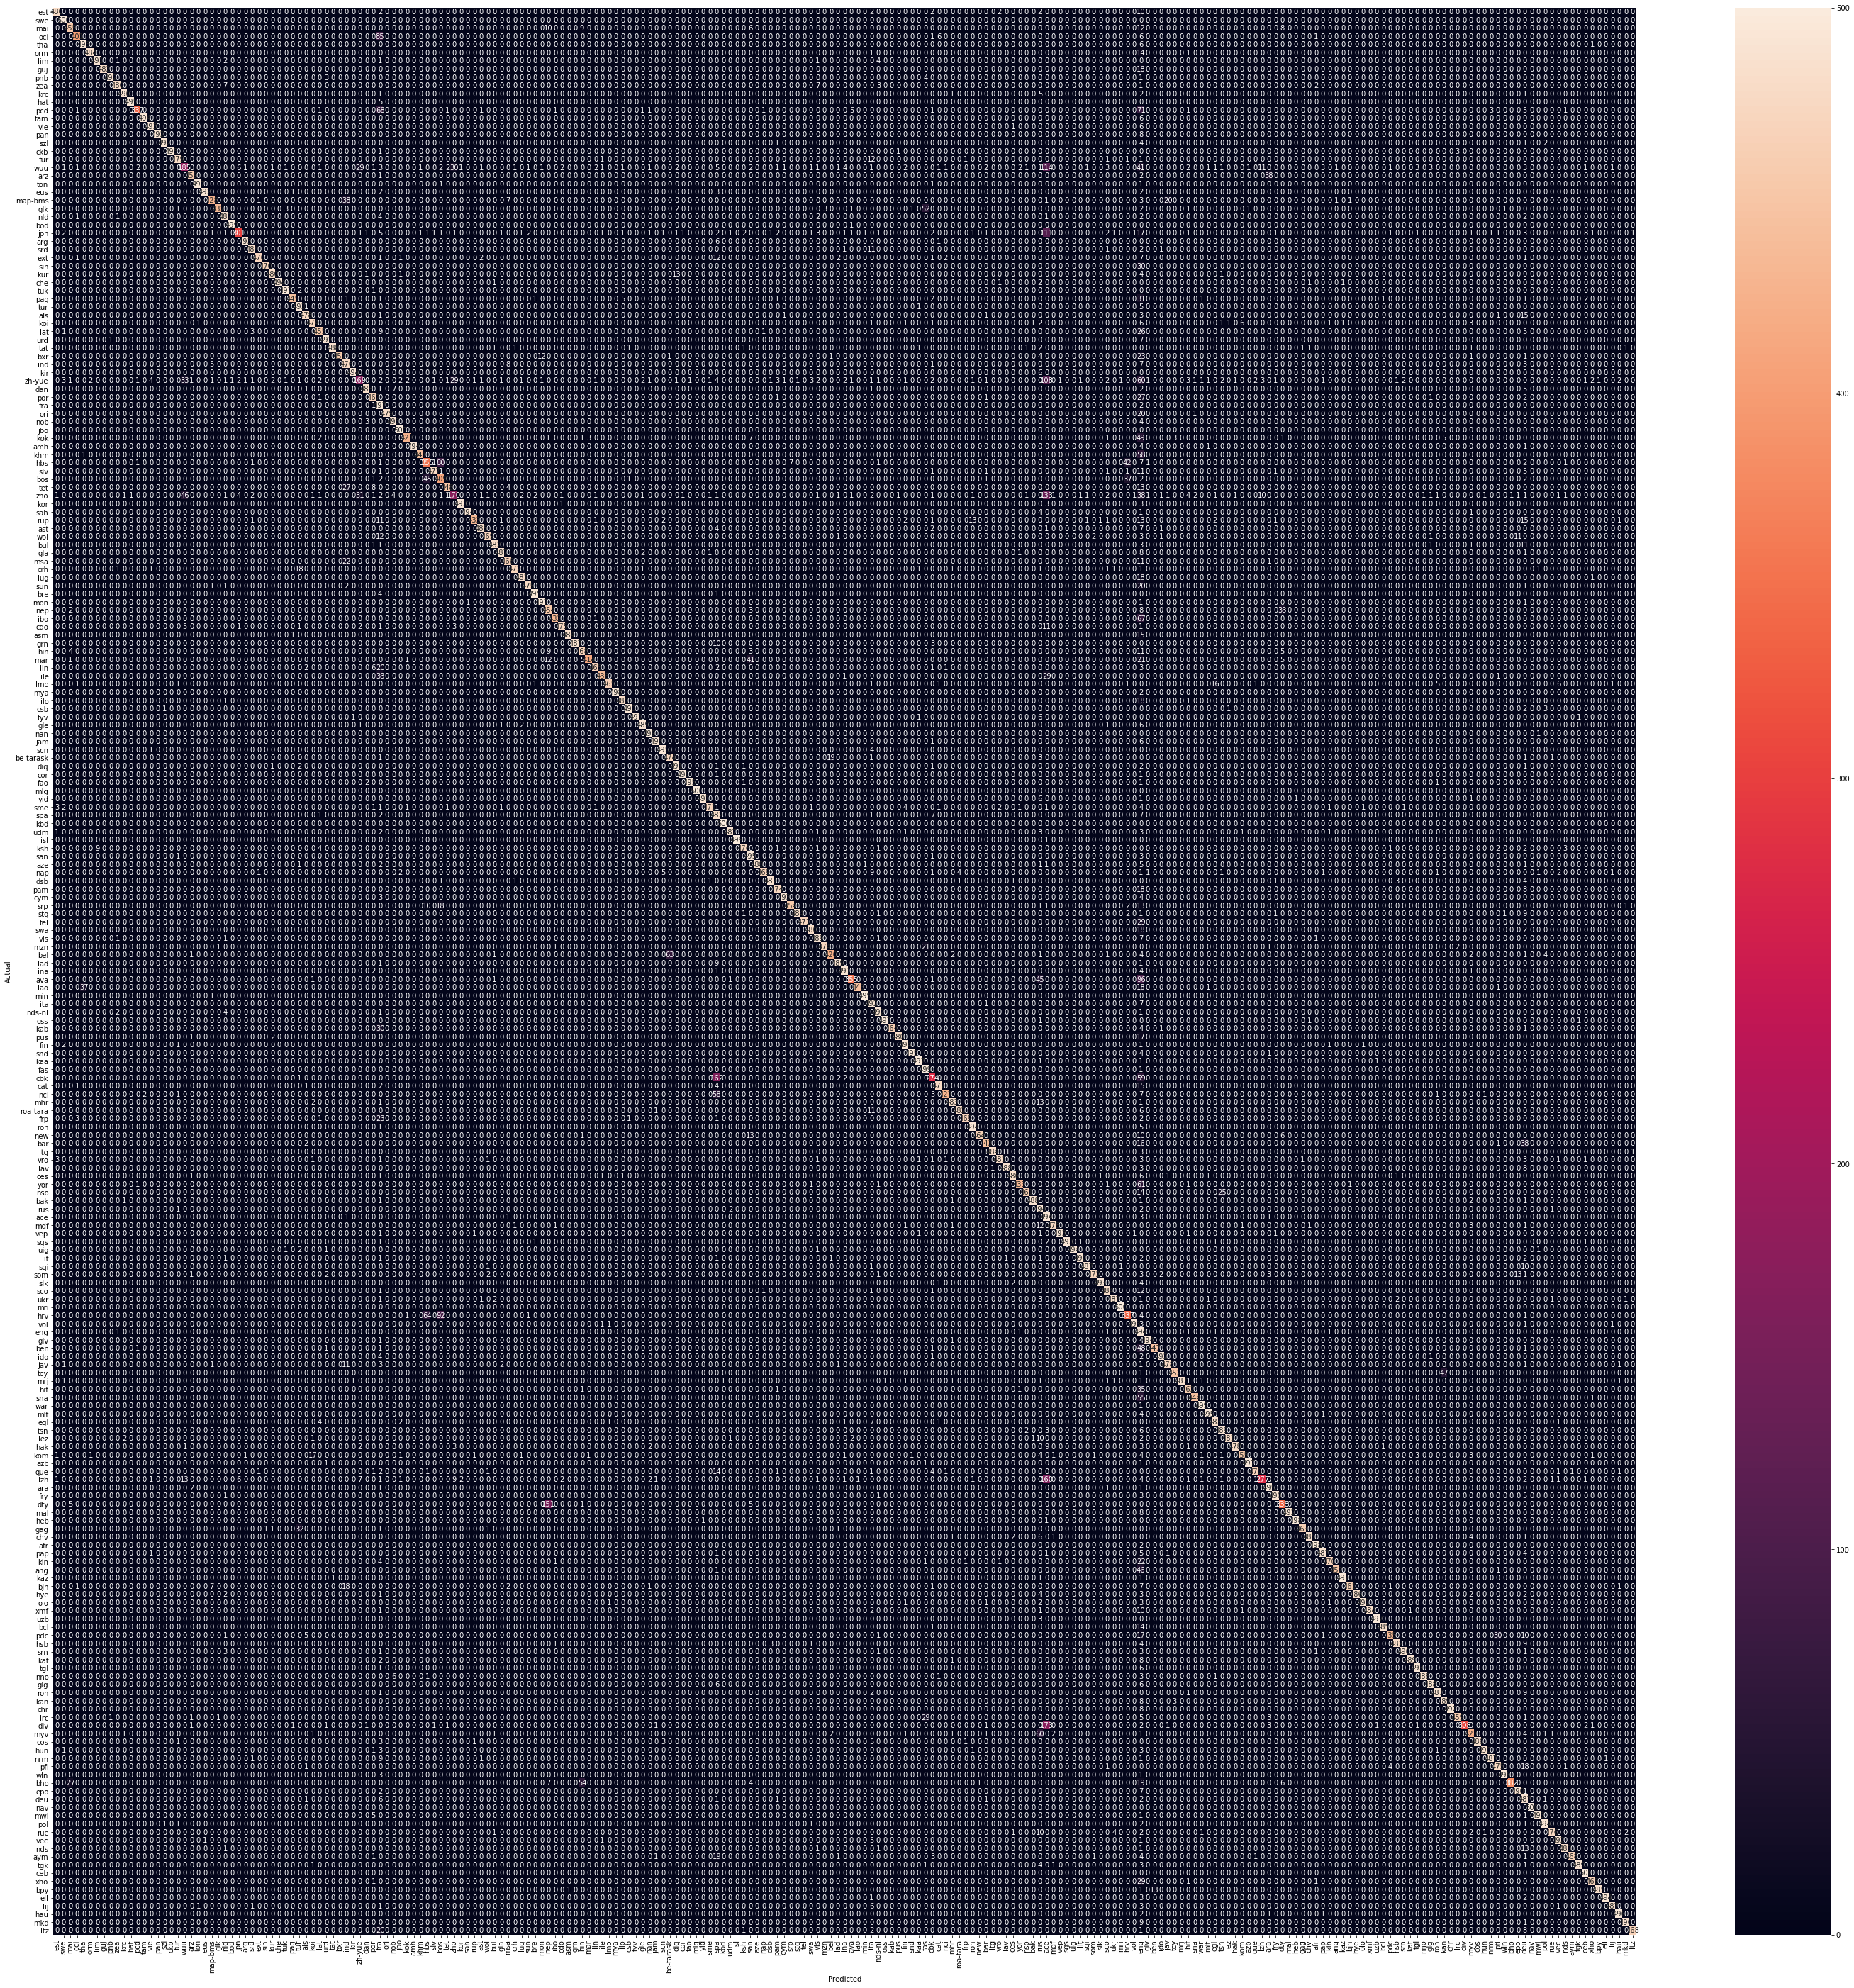
\includegraphics[width=\textwidth]{conf_mat_cv}
		%\end{adjustbox}  
		\caption{Confusion matrix for the NB-cv model}
		\label{fig:conf_mat_cv}      
	%\end{minipage}
\end{figure*}

% that's all folks
\end{document}


